% ============================================================================
% CHAPITRE 4 — SPRINT 2 : PIPELINE RAG MULTILINGUE
% ============================================================================

\section{Introduction}

Ce chapitre détaille le déroulement du Sprint~2 du projet Guidni. Ce deuxième Sprint, d'une
durée de quatre semaines (novembre 2024), est consacré à l'implémentation du pipeline RAG
(Retrieval-Augmented Generation) multilingue et de la recherche sémantique. Pour cela,
j'ai suivi le plan suivant~:
\begin{enumerate}
    \item Planning du Sprint
    \item Analyse
    \item Conception
    \item Réalisation
    \item Sprint Review
\end{enumerate}


% ────────────────────────────────────────────────────────────────
\section{Planning du Sprint~2}
% ────────────────────────────────────────────────────────────────

\subsection{Objectif du Sprint}

L'objectif du Sprint~2 est de déployer une architecture RAG multilingue capable de répondre
à des requêtes sémantiques complexes en français, anglais et arabe, sans sacrifier la latence
du backend FastAPI. Ce Sprint trouve sa genèse dans les observations de la Sprint Retrospective
précédente~: la recherche textuelle pure s'avère insuffisante pour interroger le catalogue
touristique de Djerba.

\subsection{Sprint Backlog}

\begin{table}[H]
    \centering
    \caption{Sprint Backlog --- Sprint~2}
    \label{tab:sprint2_backlog}
    \small
    \begin{tabular}{c c p{7cm} c}
        \toprule
        \textbf{ID US} & \textbf{ID Task} & \textbf{Task} & \textbf{Complexité} \\
        \midrule
        US-04 & T-2.1 & Installation et configuration de BAAI/bge-m3 (embeddings) & M \\[3pt]
        US-04 & T-2.2 & Installation du modèle bge-reranker-v2-m3 (cross-encoder) & M \\[3pt]
        US-04 & T-2.3 & Implémentation du pipeline de vectorisation des entités & L \\[3pt]
        US-04 & T-2.4 & Configuration des paramètres de chunking (512 tokens, overlap 50) & S \\[3pt]
        US-04 & T-2.5 & Implémentation du moteur de requête RAG two-stage & XL \\[3pt]
        US-04 & T-2.6 & Déport du reranking sur worker thread (asyncio.to\_thread) & M \\[3pt]
        US-04 & T-2.7 & Implémentation de la réindexation incrémentale via SQLAlchemy events & L \\[3pt]
        US-09 & T-2.8 & Endpoint \texttt{POST /admin/rebuild-index} pour reconstruction RAG & S \\[3pt]
        US-04 & T-2.9 & Tests de récupération sémantique multilingue (FR/EN/AR) & M \\
        \bottomrule
    \end{tabular}
\end{table}

\subsection{Definition of Done (DoD)}

\begin{itemize}
    \item Une requête multilingue complexe (ex.\ : \enquote{endroit romantique et calme} en
    trois langues) doit restituer des résultats sémantiquement pertinents.
    \item Le reranking cross-encoder ne doit pas bloquer la boucle d'événements (Event Loop)
    de FastAPI.
    \item L'index vectoriel est maintenu à jour automatiquement lors des modifications en base.
\end{itemize}


% ────────────────────────────────────────────────────────────────
\section{Analyse}
% ────────────────────────────────────────────────────────────────

\subsection{Diagramme de cas d'utilisation}

\begin{figure}[H]
    \centering
    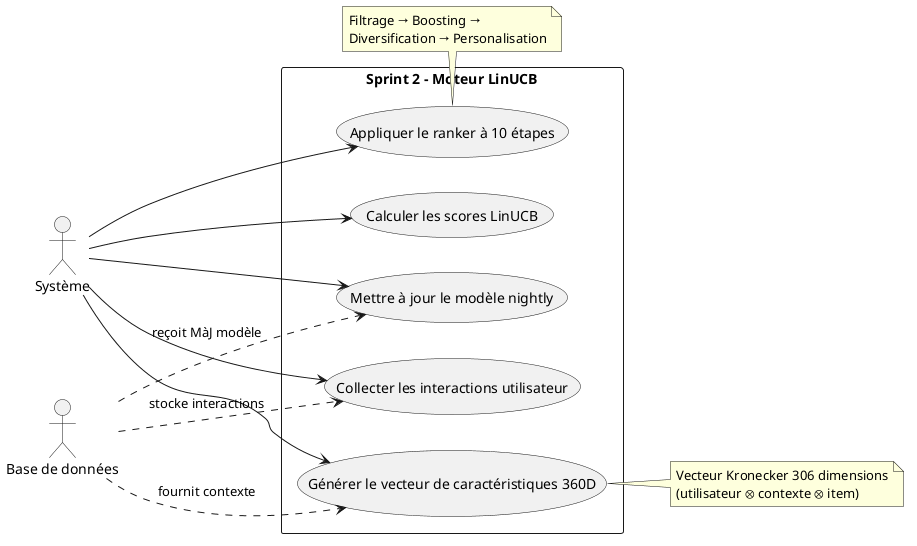
\includegraphics[width=0.85\textwidth]{diagrams/plantuml/usecase_sprint2.png}
    \caption{Diagramme de cas d'utilisation --- Sprint~2}
    \label{fig:uc_sprint2}
\end{figure}

\subsection{Description textuelle des cas d'utilisation}

\begin{table}[H]
    \centering
    \caption{Description textuelle --- CU : Effectuer une recherche sémantique RAG}
    \label{tab:cu_sprint2_1}
    \small
    \begin{tabular}{p{3cm} p{10cm}}
        \toprule
        \textbf{Champ} & \textbf{Description} \\
        \midrule
        Titre & Effectuer une recherche sémantique RAG \\[3pt]
        Acteur & Système (agent LangGraph via outil RAG) \\[3pt]
        Pré-condition & L'index vectoriel est initialisé et contient les entités indexées \\[3pt]
        Scénario nominal &
        1. L'agent appelle l'outil \texttt{rag\_search} avec une requête textuelle \newline
        2. Le moteur calcule le vecteur d'embedding via BAAI/bge-m3 \newline
        3. Les 50 candidats les plus proches (similarité cosinus) sont récupérés \newline
        4. Le cross-encoder bge-reranker-v2-m3 réordonne les candidats (sur worker thread) \newline
        5. Les Top-K résultats sont retournés avec leurs scores \\[3pt]
        Post-condition & Les résultats pertinents sont injectés dans le contexte de l'agent \\
        \bottomrule
    \end{tabular}
\end{table}

\begin{table}[H]
    \centering
    \caption{Description textuelle --- CU : Réindexer automatiquement une entité modifiée}
    \label{tab:cu_sprint2_2}
    \small
    \begin{tabular}{p{3cm} p{10cm}}
        \toprule
        \textbf{Champ} & \textbf{Description} \\
        \midrule
        Titre & Réindexer automatiquement une entité modifiée \\[3pt]
        Acteur & Système (écouteur SQLAlchemy) \\[3pt]
        Pré-condition & L'entité modifiée est de type Activity, Stay, Restaurant ou Attraction \\[3pt]
        Scénario nominal &
        1. L'administrateur modifie une entité via le frontend \newline
        2. L'événement \texttt{after\_update} est intercepté par l'écouteur SQLAlchemy \newline
        3. Une tâche asynchrone est créée via \texttt{loop.create\_task()} \newline
        4. Le vecteur d'embedding de l'entité est recalculé \newline
        5. L'entrée correspondante dans l'index vectoriel est mise à jour \\[3pt]
        Post-condition & L'index vectoriel reflète les données actualisées \\
        \bottomrule
    \end{tabular}
\end{table}


% ────────────────────────────────────────────────────────────────
\section{Conception}
% ────────────────────────────────────────────────────────────────

\subsection{Diagramme de séquence --- Recherche RAG two-stage}

Le diagramme suivant illustre le pipeline de récupération documentaire à deux étapes~: la
phase de récupération par similarité cosinus suivie du réordonnancement par cross-encoder.

\begin{figure}[H]
    \centering
    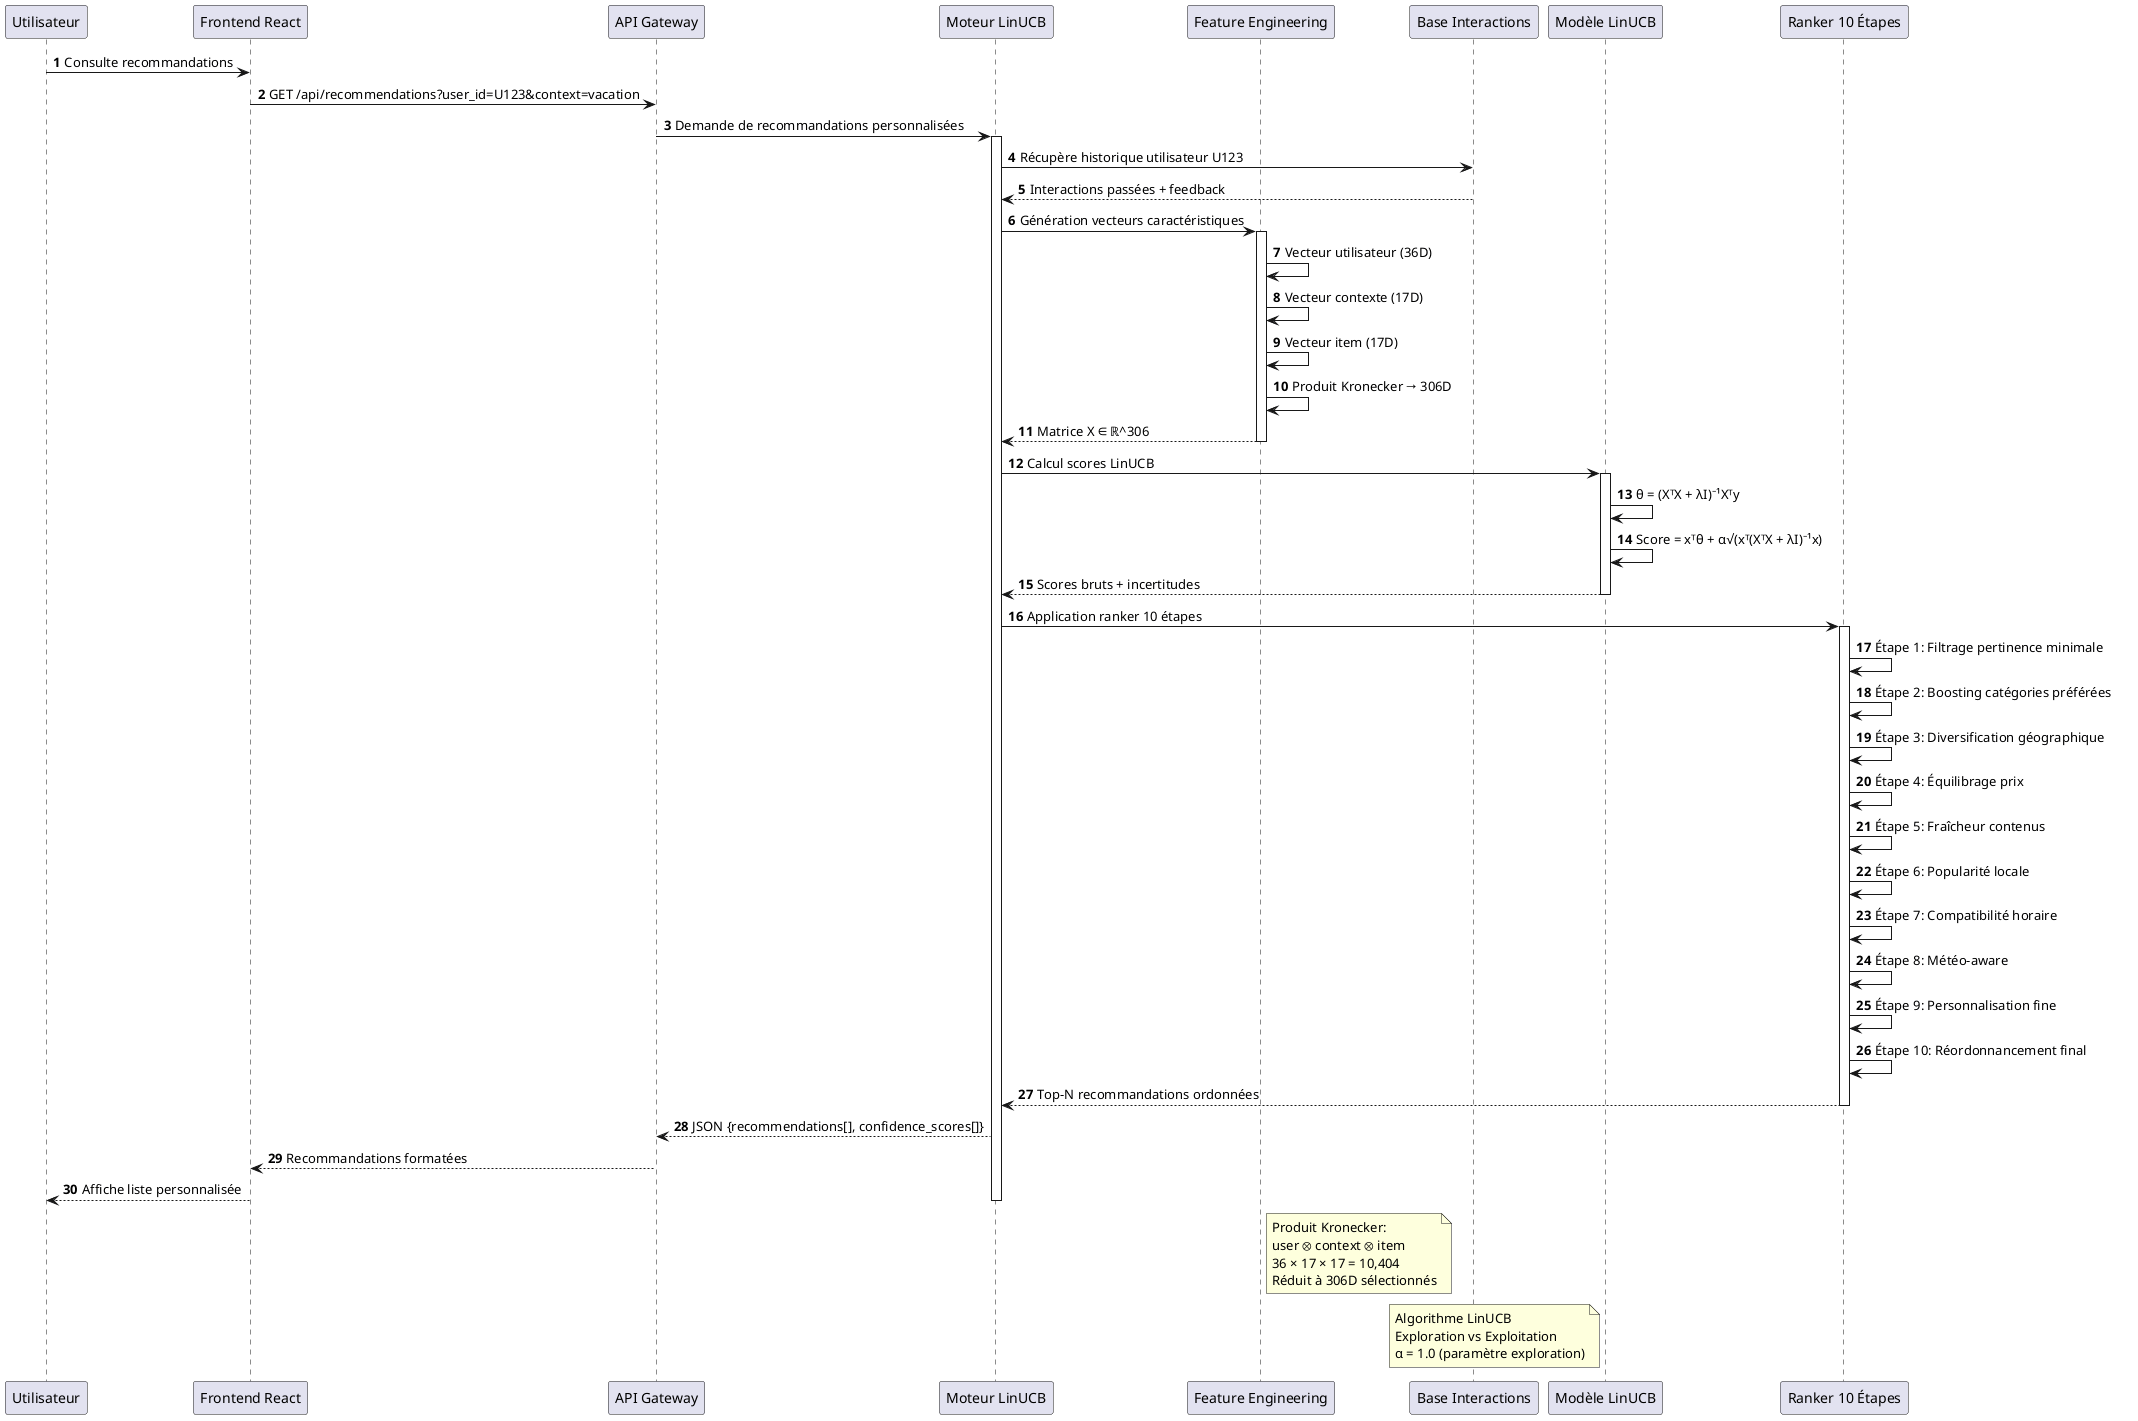
\includegraphics[width=\textwidth]{diagrams/plantuml/sequence_sprint2_primary.png}
    \caption{Diagramme de séquence --- Pipeline RAG two-stage}
    \label{fig:seq_sprint2_primary}
\end{figure}

\subsection{Diagramme de séquence --- Réindexation incrémentale}

\begin{figure}[H]
    \centering
    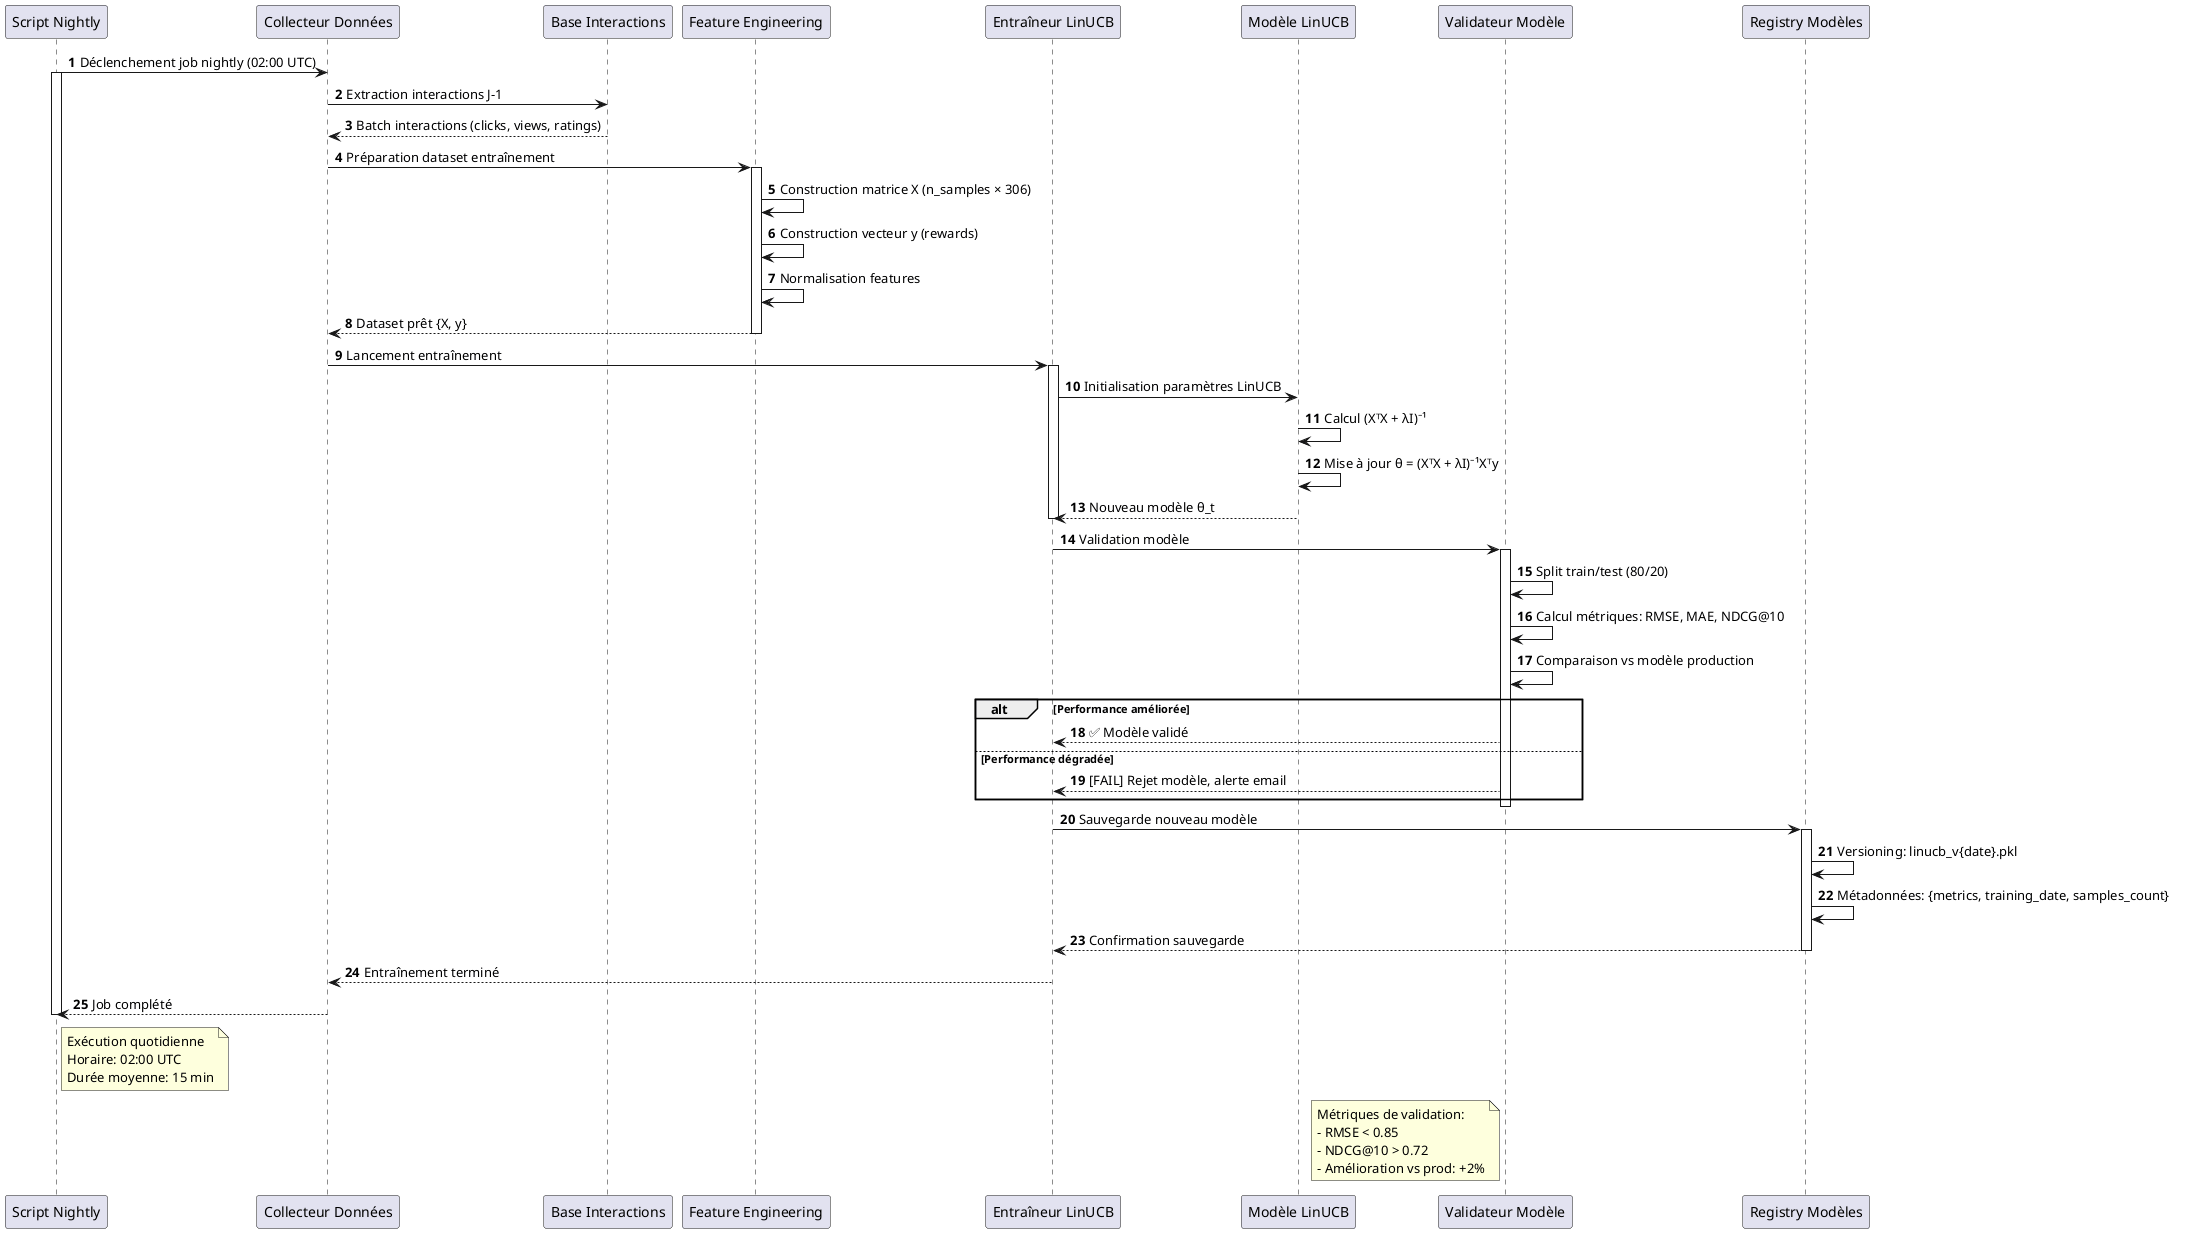
\includegraphics[width=\textwidth]{diagrams/plantuml/sequence_sprint2_secondary.png}
    \caption{Diagramme de séquence --- Réindexation incrémentale via SQLAlchemy events}
    \label{fig:seq_sprint2_secondary}
\end{figure}


% ────────────────────────────────────────────────────────────────
\section{Réalisation}
% ────────────────────────────────────────────────────────────────

\subsection{Pipeline RAG}

Le pipeline RAG a été implémenté avec les composants suivants~:

\begin{itemize}
    \item \textbf{Modèle d'embedding}~: BAAI/bge-m3 (1024~dimensions, 100+~langues), instancié
    globalement au démarrage via \texttt{initialize\_rag\_settings()}.
    \item \textbf{Paramètres de chunking}~: \texttt{chunk\_size=512}, \texttt{chunk\_overlap=50}.
    \item \textbf{Moteurs vectoriels}~: support de Qdrant et pgvector (configurable via
    \texttt{VECTOR\_ENGINE}).
    \item \textbf{Entités indexées}~: Activity, Stay, Restaurant, Attraction, Rental, Transfer.
\end{itemize}

Le pipeline de récupération s'exécute en deux étapes~: la première récupère les 50 candidats
les plus proches par similarité cosinus, la seconde applique le cross-encoder
bge-reranker-v2-m3 pour réordonner les résultats. Le calcul du reranking est déporté
sur un worker thread via \texttt{asyncio.to\_thread} pour ne pas bloquer l'Event Loop.

\begin{figure}[H]
    \centering
    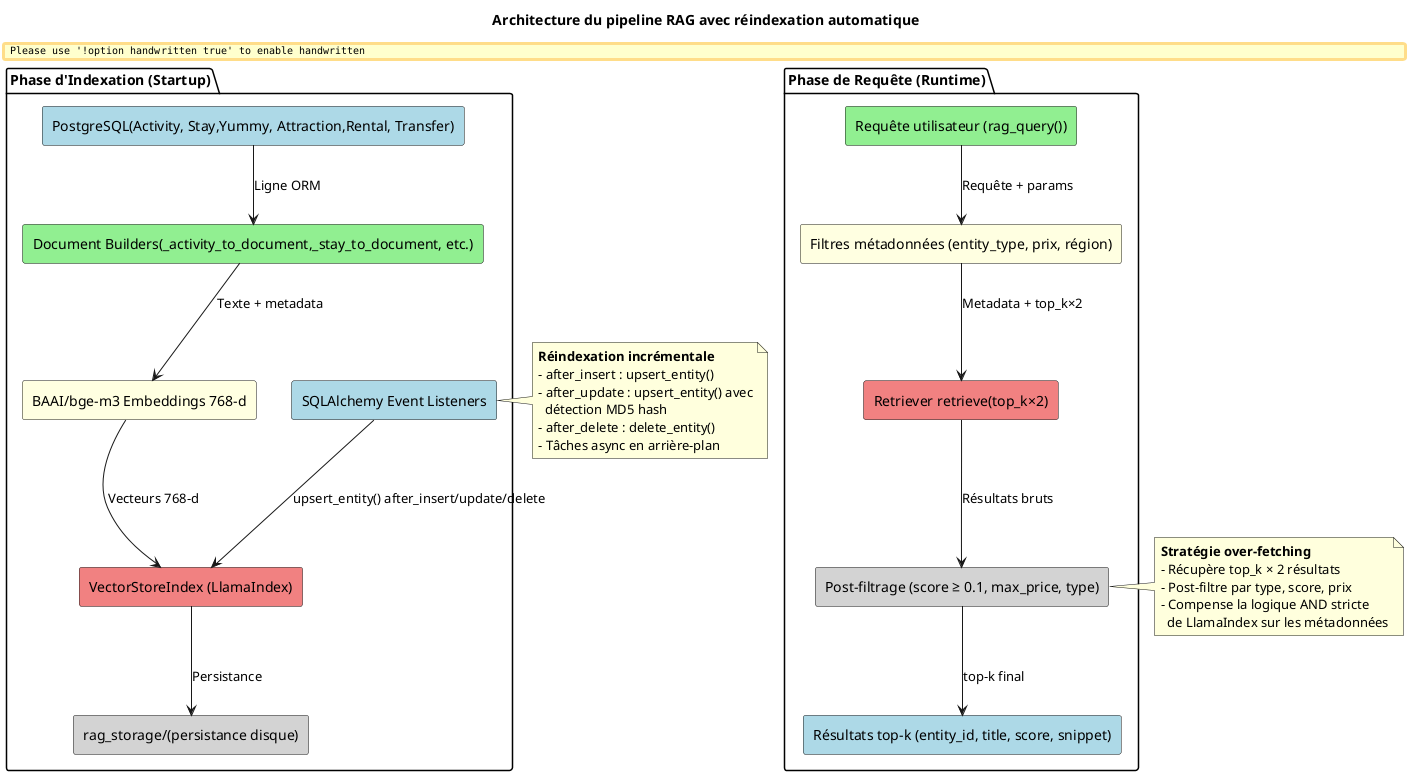
\includegraphics[width=0.85\textwidth]{diagrams/fig_02_rag_architecture.png}
    \caption{Architecture du pipeline RAG avec réindexation automatique}
    \label{fig:rag_pipeline}
\end{figure}

\subsection{Réindexation incrémentale}

Le module \texttt{db\_events.py} attache des écouteurs sur les événements
\texttt{after\_insert}, \texttt{after\_update} et \texttt{after\_delete} des six modèles
suivis. Chaque modification déclenche une tâche asynchrone en arrière-plan pour mettre à jour
le vecteur correspondant dans l'index.

\subsection{Résultats de recherche multilingue}

La figure suivante montre un exemple de recherche RAG multilingue, où une requête en français
\enquote{logement calme avec vue sur mer} retourne des résultats pertinents malgré des
descriptions en anglais et en arabe dans la base.

\begin{figure}[H]
    \centering
    
\includegraphics[width=\textwidth]{diagrams/screen_04_rag_search_result.png}
    \caption{Résultats de recherche RAG multilingue}
    \label{fig:screen_rag}
\end{figure}

\subsection{Interface d'administration}

L'endpoint \texttt{POST /admin/rebuild-index} permet à l'administrateur de déclencher une
reconstruction complète de l'index vectoriel. La figure suivante montre la réponse de
l'endpoint après une reconstruction réussie.

\begin{figure}[H]
    \centering
    
\includegraphics[width=\textwidth]{diagrams/screen_A4_admin_rebuild.png}
    \caption{Interface de reconstruction de l'index RAG (endpoint admin)}
    \label{fig:screen_admin_rebuild}
\end{figure}


% ────────────────────────────────────────────────────────────────
\section{Sprint Review}
% ────────────────────────────────────────────────────────────────

Lors de la Sprint Review concluant le Sprint~2, la plateforme Guidni, renforcée du système RAG,
a été testée avec des requêtes multilingues complexes. En particulier, la requête
\enquote{logements calmes avec une vue en hauteur pour jeunes mariés}, formulée en trois
langues distinctes, a effectivement retourné des offres pertinentes, prouvant le bilinguisme
cognitif du modèle bge-m3. L'encadrant a validé l'intégration fluide du système RAG.

Lors de la Sprint Retrospective, l'équipe a identifié le besoin d'un agent conversationnel
capable d'orchestrer les outils de recherche RAG de manière autonome, justifiant le Sprint~3
consacré à la machine à états LangGraph.


% ────────────────────────────────────────────────────────────────
\section*{Conclusion}
\addcontentsline{toc}{section}{Conclusion}

Le Sprint~2 a permis d'implémenter le pipeline RAG multilingue complet, incluant les
embeddings BAAI/bge-m3, le cross-encoder de réordonnancement, et la réindexation incrémentale
via les événements SQLAlchemy. Les tests ont confirmé la capacité du système à traiter des
requêtes sémantiques complexes en trois langues. Le Sprint~3 sera consacré à l'implémentation
de l'agent LLM et de la machine à états LangGraph pour la planification conversationnelle.
